% main text for the telluric section in keck.tex
%%%%%%%%%%%%%%%%%%%%%%%%%%%%%%%%%%%%%%%%%%%%%%%%%%%%%%%%%%%%%%%%%%%%%%%%%%%%
%%%%%%%%%%%%%%%%%%%%%%%%%%%%%%%%%%%%%%%%%%%%%%%%%%%%%%%%%%%%%%%%%%%%%%%%%%%%
\subsection{Introduction}\label{keck:telluric:intro}

Traditionally, telluric contamination is not considered as problematic
for precise RV in the optical. It is certainly a sever source of
spectral contamination and a bottleneck for achieving higher RV
precision in the near infra-red (NIR) region (e.g.,
\citealt{2010ApJ...713..410B}), where a large number of deep water and
methane lines reside. However, there is only a small wavelength
range in the optical that has deep telluric lines, and typically such
regions are simply thrown out for the purpose of precise RV analysis,
either by giving them zero weights in the cross correlation masks (for
ThAr calibrated spectra, e.g., \citealt{2002A&A...388..632P}) or
flagging them as bad pixels (for iodine calibrated spectra, e.g., for
\keck).

Recently, the works by \cite{artigau2014} and \cite{cunha2014} have
characterized and mitigated the effects of telluric contamination in
the precise RV data taken by the ThAr-calibrated HARPS-S.
\cite{cunha2014} focuses on the issues with ``micro-telluric" lines
(shallow telluric absorption lines with $<1$-3\% depths;
Figure~\ref{telluric:fig:telluric}), which are recognized for the
first time. \cite{cunha2014} fit and then divide out the telluric
lines in the observed spectra using synthetic telluric spectra
generated by the LBLRTM package (Line-By-Line Radiative Transfer
Model, \citealt{lblrtm}; with line lists from HIgh-resolution
TRANsmission molecular absorption database, or HITRAN,
\citealt{hitran2013}) and also TAPAS \citep{tapas}, which is a more
user-friendly but less flexible package wrapper using LBLRTM. They
concluded that the micro-tellurics have an impact (defined as the
root-mean-square, RMS, of difference between RVs before and after
micro-telluric removal) of $\sim$10-20 cm/s for G stars observed with
low to moderate air masses, but the impact can be substantial in some
cases to up to $\sim$0.5-1 m/s.

\cite{artigau2014} uses principal component analysis (PCA) to
empirically correct for telluric lines in HARPS-S data (both
micro-tellurics and the deep lines in the $\sim$630~nm region), and
combined PCA with rejection masking, they reduced the RV RMS by
$\sim$20~cm/s (and more significantly for the $\sim$630~nm
region). More recently, \cite{2016AAS...22713719S} characterized the
effects of telluric contamination and effectiveness of some typical
remedies (masking and modeling) for emission line-calibarated spectra
for the optical, broad optical (300-900~nm), and NIR. Their conclusion
for the optical region is similar to the results in \cite{artigau2014}
and \cite{cunha2014}.

This section characterizes and corrects for the adverse effects of
telluric contamination under the context of iodine-calibrated precise
RV, especially for the micro-telluric lines. We first quantify the
effects of tellurics in RV precision and accuracy through simulations
(Section~\ref{keck:telluric:impact}), and then we talk about remedies
and their effectiveness to eliminate the adverse effects in real
observed data (Section~\ref{keck:telluric:remedies}). We summarize our
recommendations for treating telluric contamination in
iodine-calibrated RV data in Section~\ref{keck:telluric:summary}.


%----------------------------------------------------------------
% Plot showing micro-telluric lines
% made by ~/Exo../Keck../plots_general/spec_plot.pro
\begin{figure}
\includegraphics[scale=0.5]{telluric/tellurics_all.eps} 
\caption{Telluric lines in the iodine region are mostly shallow water
lines, with some moderately deep water lines near 5900\AA\ and very
deep oxygen lines near 6300\AA. The insert plot is showing the
pervasiveness of micro-telluric lines, i.e.~$\leq$1--3\% in depths.
\label{telluric:fig:telluric}}
\end{figure}
%----------------------------------------------------------------



%%%%%%%%%%%%%%%%%%%%%%%%%%%%%%%%%%%%%%%%%%%%%%%%%%%%%%%%%%%%%%%%%%%%%%%%%%%%
%%%%%%%%%%%%%%%%%%%%%%%%%%%%%%%%%%%%%%%%%%%%%%%%%%%%%%%%%%%%%%%%%%%%%%%%%%%%
\subsection{Characterize the Impacts of Micro-tellurics on RV
  Precision via Simulation}\label{keck:telluric:impact} 

% why Keck, why 185144 and 10700
To evaluate the impacts of micro-tellurics (referred to often simply
as ``tellurics'' below), we performed end-to-end simulation of \keck\
data and analysis process on RV standard stars in order to isolate
error sources. We use \keck\ data to for our study because Keck has
the highest RV precision among all iodine-calibrated spectrometers,
and it also has long observing baselines on a number of RV standard
stars. RV standard stars are bright and quite stars which do not host
known planets, and thus exhibit the smallest RV variation in both
short term and long term. Their data are often good diagnostic tools
for identifying RV systematics. For our study, we used and simulated
\keck\ RV spectra on two standard stars, $\sigma$ Draconis (HD 185144)
and $\tau$ Ceti (HD 10700), which are benchmark classics in precise RV
work.

% more on the two stars 
HD 185144 (spectral type G9V, per Simbad) has 712 \keck\ observations,
with RV RMS $=$ 2.57 m/s, and it has a relatively small barycentric
velocity (often referred to as the barycentric velocity correction, or
BC; see Chapter~\ref{chap:doppler}) span, $[-4.7,\ 4.6]$ km/s, because
it is near the north ecliptic pole. HD 10700 (spectral type G8.5V) has
623 observations, with RMS $=$ 3.05 m/s, and its BC span is $[-27.8,\
26.8]$ km/s. The RV RMS numbers quoted here come from reductions using
our version of CPS Doppler pipeline, and they are larger than the RMS
values from the most up-to-date CPS pipeline due to some recent
improvements in the CPS version. The most recent CPS inventory (as of
April 2016) also has a few new observations on these two stars.

We describe how we simulated our data and used them to characterize
the impacts of tellurics in Section~\ref{keck:telluric:method}, and
then lay out our results in Section~\ref{keck:telluric:results}.


%%%%%%%%%%%%%%%%%%%%%%%%%%%%%%%%%%%%%
\subsubsection{Methodology of the Simulation}\label{keck:telluric:method}

% how we approach the problem with simulation
The overall strategy is to bring out the effects of telluric
contamination by comparing the extracted RVs from pairs of simulated
observations: one with telluric absorption, and the other one in the
pair without. For example, for HD 185144, we simulated two spectra for
each of the 712 real observed spectrum. We then had two sets of
simulated observations, one free of tellurics and one contaminated
with tellurics. Next we ran the Doppler code on each set of 712
spectra to extract RVs from them, and for the set with tellurics we
used telluric-contaminated DSST and a telluric-free DSST for the
telluric-free spectra. \\

% how we simulated the spectrum
Below is our recipe for simulating \keck\ spectra and DSSTs:
\begin{enumerate}
\item Generate a synthetic spectrum for the target star using
  Spectroscopy Made Easy (SME;
  \citealt{valentipiskunov1996,valentifischer2005}; the SME spectra are
  kindly provided by Jason Curtis). We refer to this spectrum as the
  input synthetic spectrum or the SME spectrum.
\item Based on the SME spectrum, generate a DSST for the target
  star. First, we redshift the SME spectrum so that it has the same
  barycentric velocity as the real DSST of the target star. Then we
  break the SME spectrum into chunks as defined by the real DSST (an IDL
  structure) of this target star.
\item Run TERRASPEC, a versatile software for synthesizing telluric
  spectrum (it is a wrapper around the HITRAN line list and the LBLRTM
  package), to generate a telluric absorption spectrum using a typical
  Mauna Kea atmospheric condition in the summer, with precipitable water
  vapor (pwv) 1~mm (a little bit more humid than Keck's usual
  condition), and oxygen column density that is consistent with the
  altitude of the real DSST observation. We multiply this synthetic
  telluric spectrum with the SME spectrum to make a
  telluric-contaminated DSST.
\item Loop through each real observed spectra of the target star, and
  simulate a pair of observations following this recipe:
  \begin{enumerate}
  \item Shift the SME spectrum to have the same barycentric velocity
    as the star at the epoch of the real observation (i.e., assuming
    intrinsic stellar velocity is zero).
  \item Generate a continuous wavelength solution for each echelle
      order based on the best-fit wavelength solution for the real
      spectrum. 
  \item Re-sample the SME spectrum and the iodine atlas onto a
    wavelength grid that is four times finer than the wavelength
    solution grid. Multiply the stellar spectrum with the iodine
    atlas.
  \item To add telluric contamination: multiply the simulated spectrum
    with a telluric absorption spectrum generated with TERRASPEC, again
    for typical Mauna Kea summer, with pwv $=$ 1~mm, and oxygen column
    density that is consistent with the altitude of the real observation.
  \item Determine the IP for each echelle order with two options: (1)
    a single Gaussian with $\sigma=1.7$ pixel, matching the \keck\
    resolution; (2) a sum-of-Gaussian IP derived using the average IPs for
    each echelle order. We will explain these two options later in the
    text.
  \item Convolve each order of the stellar$\times$iodine spectrum with
    the IP.
  \item Fit for the blaze function for each order of the real observed
    spectrum with a third-order polynomial using the top 1\% of the flux,
    and multiply the simulated spectrum so that they have matching ``blaze
    functions''. This also ensures that the simulated spectrum has the
    same photon counts as the real one.
  \item Add photon noise according to Poisson statistics, when
    desired.
  \end{enumerate}
\item Generate a separate data log file for each set of simulated of
  observations under the same conditions (i.e., telluric choice, IP choice,
  photon-noise choice).
\end{enumerate}

% different sets of simulations
To isolate the problem of tellurics, we first simulated spectra free
of photon noise and with a simple single Gaussian IP for the
spectrograph ($\sigma = 1.7$ pixels to match the \keck\
resolution). When extracting RVs for such sets of simulated spectra,
we fixed the IPs to the same as input and only fitted for three free
parameters. This removes the errors induced by photon noise and
uncertainties in IP fitting (which, after all, involves 12 additional
free parameters). We then added the Poisson noise to the spectra, but
still using simple and fixed IPs, to see how the effects will change
in cases with limited-SNR (as opposed to infinite SNR). Next, we used
complex IPs, the same ones as the best-fit sum-of-Gaussian IPs found
for real spectra, and float the IP parameters when extracting RVs. The
conditions and results of these three pairs of simulations are listed
in Table~\ref{telluric:tab:simulation}, and also illustrated in
Figure~\ref{telluric:fig:sim}. These results show the impacts of
telluric contamination on \keck\ data, which is discussed in the
following subsection.


%----------------------------------------------------------------
% Table: RV RMS for various simulations
\renewcommand{\arraystretch}{1.2} % more row spacing for the table
\begin{deluxetable}{ccccl}
\tabletypesize{\scriptsize}
\tablecaption{List of Simulations
\label{telluric:tab:simulation}}
\tablewidth{\textwidth}
\tablehead{
  \colhead{Simulation Conditions} & \colhead{Tellurics?} &
  \colhead{185144 RMS} &
  \colhead{10700 RMS} &
  \colhead{More Details in} 
}
\startdata
No photon noise, & No & 0.62 m/s & 1.95 m/s\tablenotemark{c} & Section~\ref{keck:telluric:results} \\ 
simple, fixed IPs & Yes & 1.21 m/s & 2.42 m/s\tablenotemark{c} & top
panels, Figure~\ref{telluric:fig:sim} \\ 
\hline
Poisson noise, & No & 2.11 m/s\tablenotemark{c} & 2.54 m/s\tablenotemark{c} & Section~\ref{keck:telluric:results} \\
simple, fixed IPs\tablenotemark{a} & Yes & 2.12 m/s\tablenotemark{c} & 2.81 m/s\tablenotemark{c} &
middle panels, Figure~\ref{telluric:fig:sim} \\ 
\hline
Poisson noise, & No & 1.22 m/s & 1.35 m/s & Section~\ref{keck:telluric:results}\\
complex, floating IPs,\tablenotemark{a} & Yes & 1.29 m/s & 1.44 m/s &
bottom panels, Figure~\ref{telluric:fig:sim} \\ 
\hline
Poisson noise, & No & 1.27 m/s & 1.43 m/s &Section~\ref{keck:telluric:masking} \\
complex, floating IPs, & Yes & 1.27 m/s & 1.43 m/s & Figure~\ref{telluric:fig:dsstmask} \\
masking the telluric pixels\tablenotemark{a} & & & & Table~\ref{telluric:tab:rmsmasking}  \\
\hline 
Poisson noise, & pwv $=$ 0.5, 0.9 & 1.28, 1.22 m/s & 1.32, 1.30 m/s &
Section~\ref{keck:telluric:neid} \\ 
complex, floating IPs, & pwv $=$ 1.0, 1.1 & 1.25, 1.23 m/s & 1.33, 1.31
m/s & Figure~\ref{telluric:fig:neid} \\ 
modeling tellurics\tablenotemark{b} 
\enddata
\tablenotetext{a}{With pairs of simulated spectra with or without
  tellurics and each pair has the same Poisson noise added.}
\tablenotetext{b}{Telluric lines added with pwv $=$ 1~mm, and we
  extracted RVs using pwv $=$ 0.5, 0.9, 1.0, 1.1~mm to access how
  accurately/precisely one needs to model the tellurics.}
\tablenotetext{c}{These simulations suffer from severe numerical and
  algorithmic errors for reasons not yet fully understood.}
\end{deluxetable}
%----------------------------------------------------------------




%%%%%%%%%%%%%%%%%%%%%%%%%%%%%%%%%%%%%
\subsubsection{Results of the Simulation}\label{keck:telluric:results}

%----------------------------------------------------------------
% Telluric effect, no photon noise
% plot made by ~/Exo.../Keck.../simulate.../msplot.pro
\begin{figure}
\subfloat{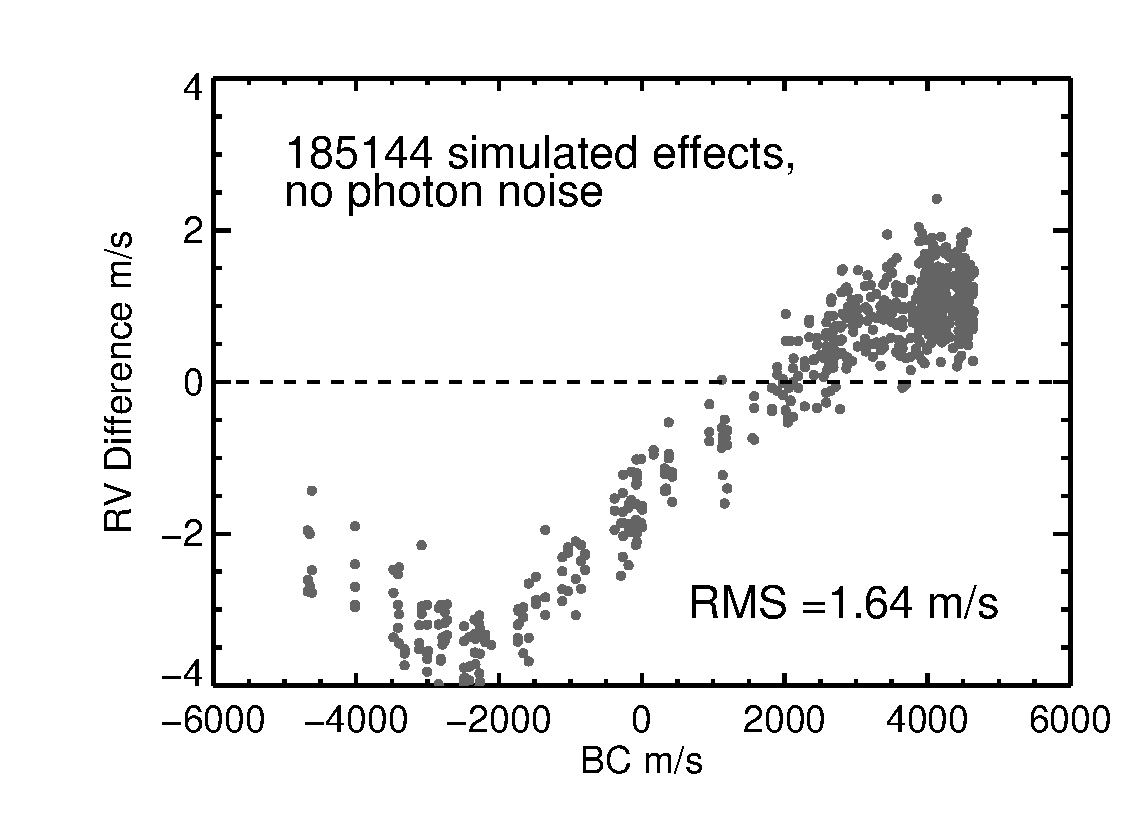
\includegraphics[scale=0.38]{telluric/185144-rv-bc-rja01-rjb01.eps}}
\subfloat{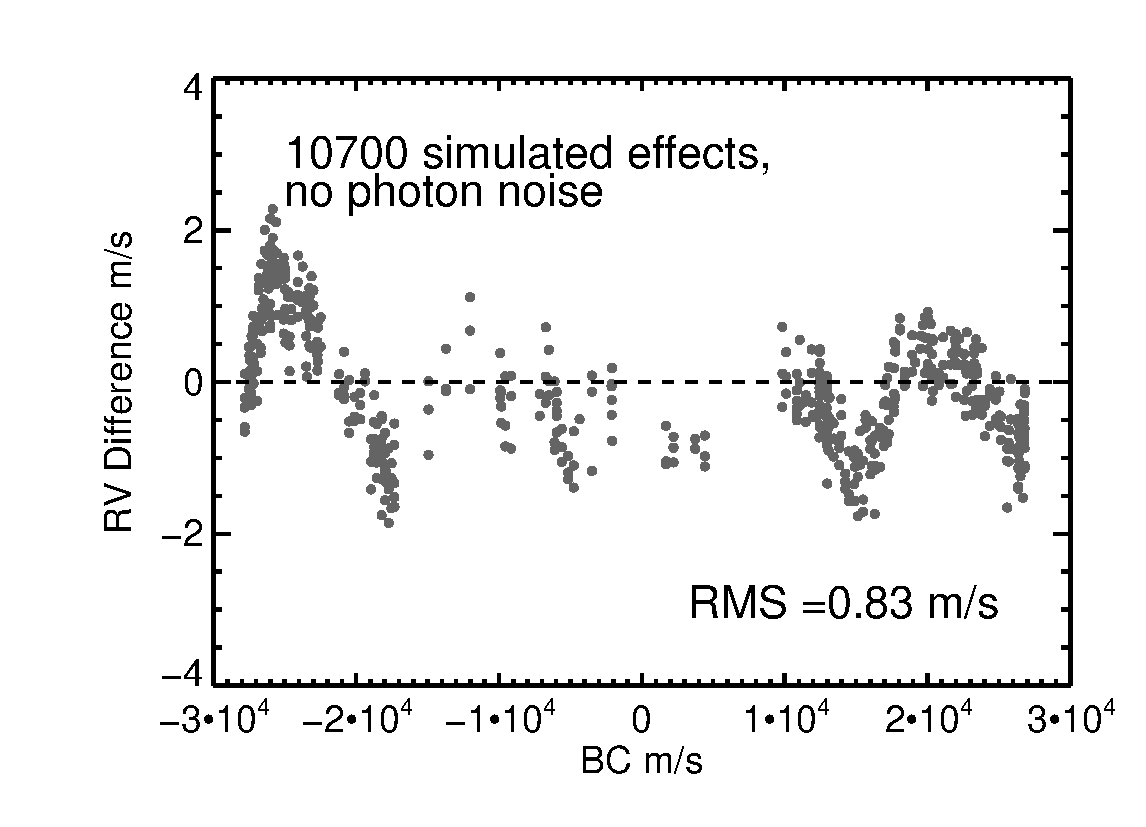
\includegraphics[scale=0.38]{telluric/10700-rv-bc-rja01-rjb01.eps}}\
\subfloat{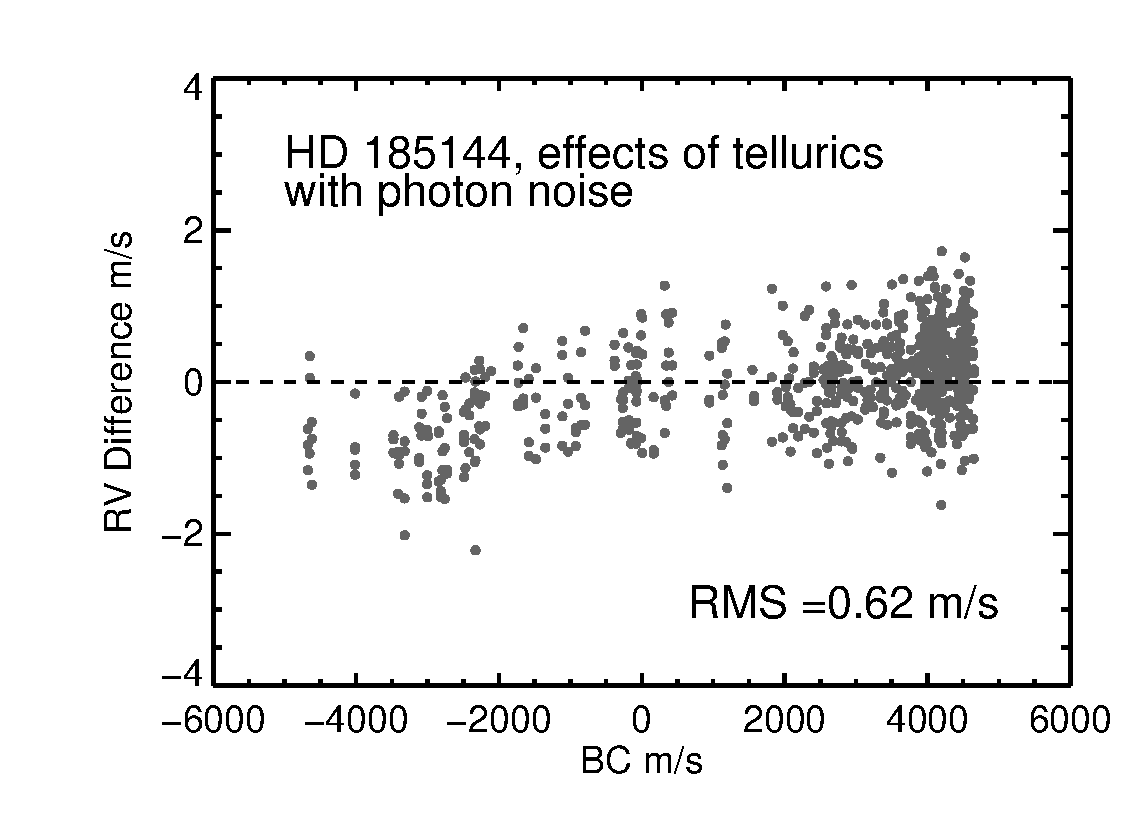
\includegraphics[scale=0.38]{telluric/185144-rv-bc-rjc01-rjd01.eps}}
\subfloat{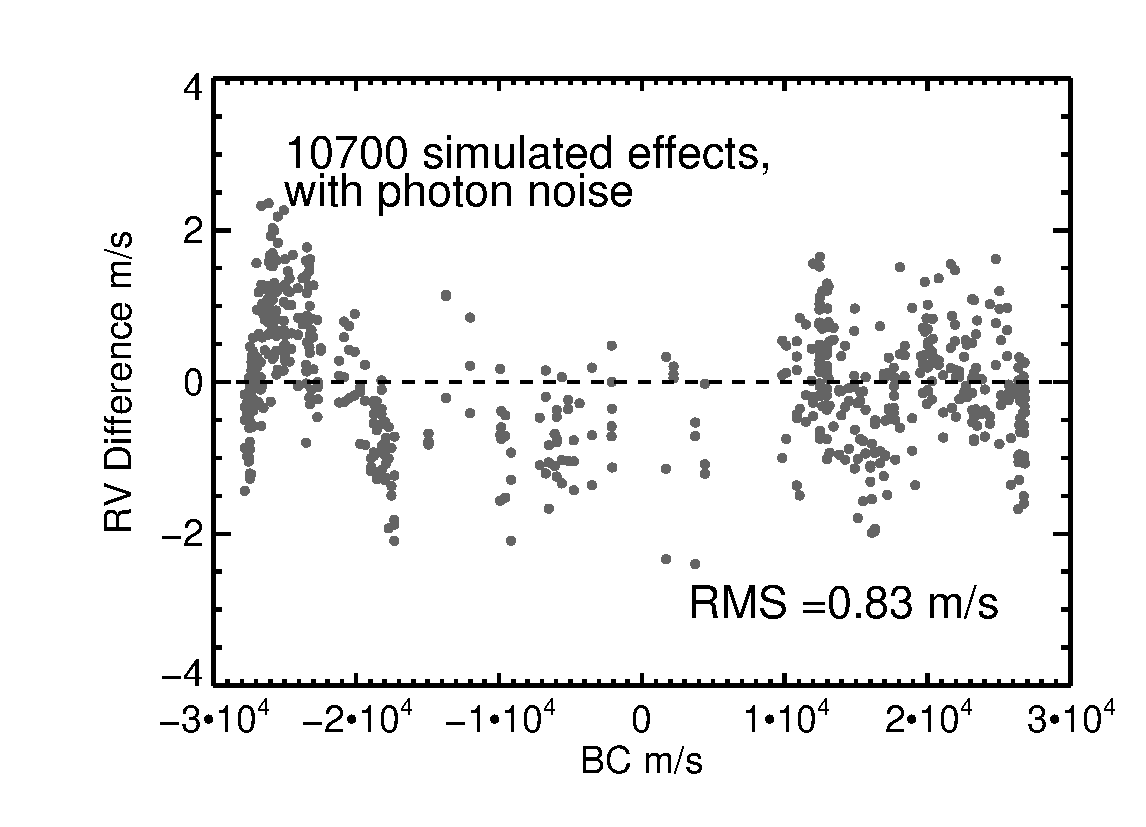
\includegraphics[scale=0.38]{telluric/10700-rv-bc-rjc01-rjd01.eps}}\
\subfloat{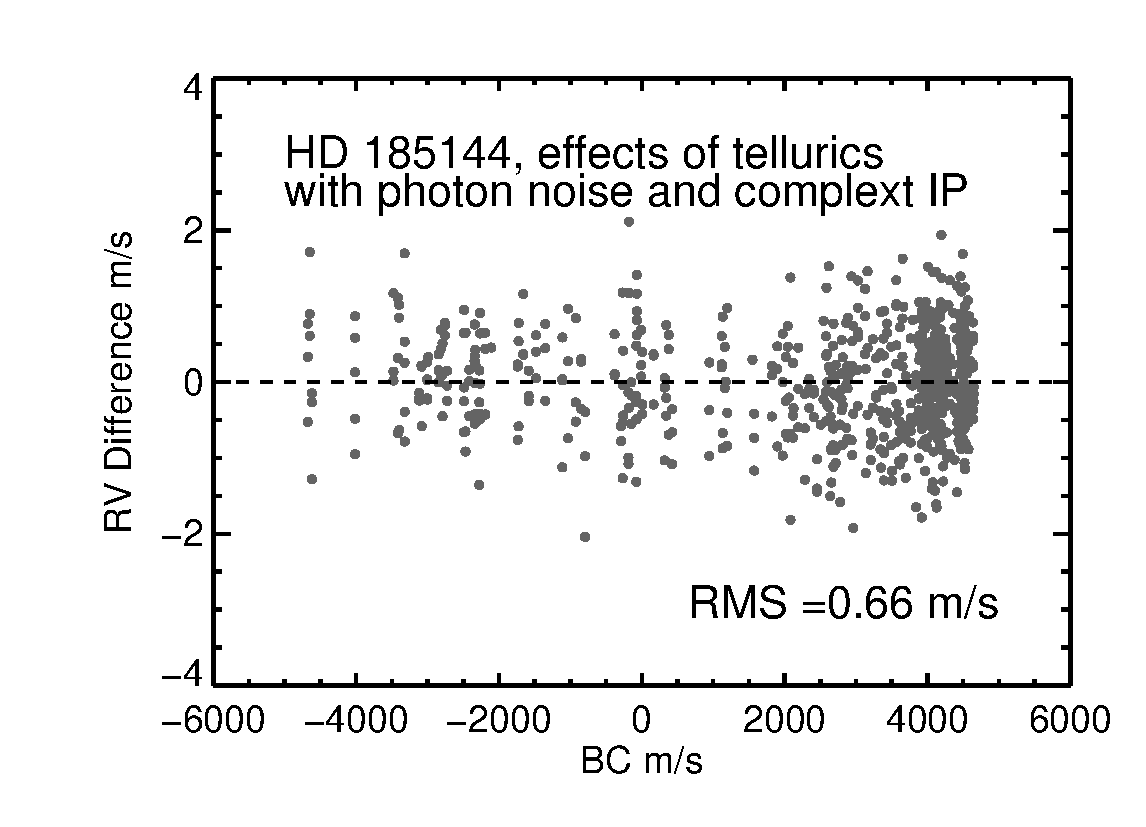
\includegraphics[scale=0.38]{telluric/185144-rv-bc-test0-test1.eps}}
\subfloat{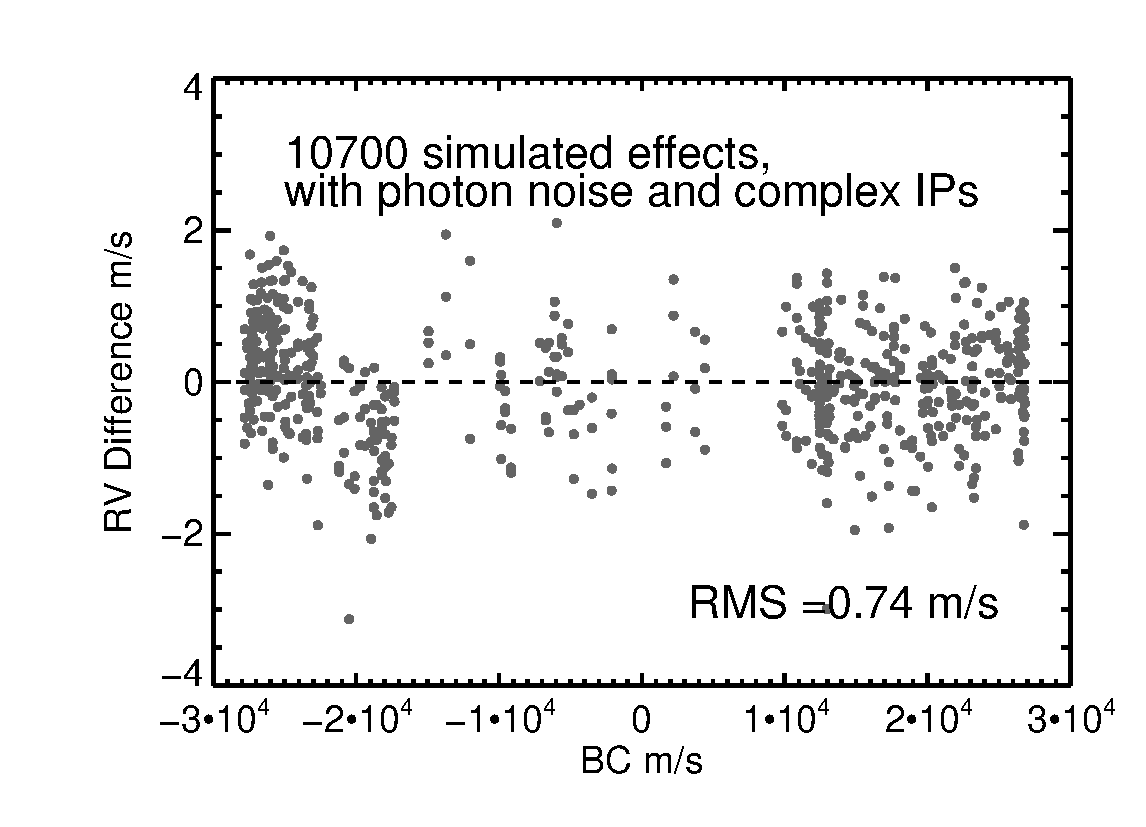
\includegraphics[scale=0.38]{telluric/10700-rv-bc-test0-test1.eps}}\
\caption{Effects of telluric lines manifested as correlation between
  RV and BC. Each point represents the difference in RV estimates for
  a pair of simulated spectra: one without telluric absorption, and
  one with telluric absorption on top of the stellar and iodine
  spectra. {\bf Top 2 panels:} To isolate the effects of telluric
  lines, the simulated spectra used for this plot do not have Poisson
  noise added, and they have simple one-component Gaussian IPs which
  have fixed width and thus the IP parameters are all fixed to the
  true values in the RV extraction. {\bf Middle 2 panels:} same as the
  top panels, but for simulated spectra with Poisson noise (same noise
  for the telluric and non-telluric spectrum pairs; and still the same
  simple IPs). {\bf Bottom 2 panels:} same as above, but for simulated
  spectra with Poisson noise and complex IPs that are similar to the
  ones in actual observations. IP parameters are not fixed in this
  case, so the code is fitting 12 additional parameters for the IP on
  top of the 3 for wavelength solution and Doppler shift (see
  Chapter~\ref{chap:doppler} for more details on the code).
\label{telluric:fig:sim}}
\end{figure}
%----------------------------------------------------------------

% no photon noise
Figure~\ref{telluric:fig:sim} illustrates the effects of telluric
contamination under different conditions. The top panels are RV
differences between the simulated spectrum pairs with infinite SNR and
perfectly known IPs, which might somewhat represent the capability of
future precise RV instruments. These two plots highlight the net
effects of telluric contamination: they cause large biases in RV
estimates, which manifest as strong RV-BC correlations or
trends. These biases clearly can not be fully corrected by the
statistical weighting or ``vanking'' procedure in the Doppler code.

% adds photon noise?
Interestingly, when we added in photon noise (middle panels of
Figure~\ref{telluric:fig:sim}), the effects of telluric contamination
are washed out significantly. This is probably because for individual
chunks, the RV scatter caused by photon noise washes out the scatters
and biases induced by tellurics, and chunks with tellurics will have a
larger RV RMS compared with telluric-free chunks. Vanking then is able
to identify telluric-contaminated chunks and assigns them smaller
weights, thus reducing the impacts of telluric contamination.

% adds complex IP
When using complex IPs and fitting for IPs in RV extraction (bottom
panels of Figure~\ref{telluric:fig:sim}), the effects of telluric
contamination are further washed out, as we are adding in more
errors. We can barely see any RV-BC correlation in the case of HD
185144 and only some in HD 10700.

% tellurics add RV RMS
The RV-BC correlations shown in Figure~\ref{telluric:fig:sim} will
translate into spurious peaks in the periodograms of the target star,
and such spurious peaks will have periods around a sidereal year and
its harmonics. This is very damaging for the search of exoplanets in
the Habitable Zone around Sun-like stars, which would have periods
around 360 days. Besides these spurious signals, telluric
contamination also causes increases in RV RMS. In all cases of
telluric-free and telluric-contaminated simulation pairs, the RV RMS
is larger for the telluric-contaminated case
(Table~\ref{telluric:tab:simulation}). The RMS numbers written in
Figure~\ref{telluric:fig:sim} represent the amount of RV RMS added (in
quadrature) because of telluric contamination (again, the spectrum
pairs are same-noise pairs -- they only differ in terms of having or
not having telluric lines). These numbers also represent a RV RMS
floor set by the telluric contamination: for example, if we ignore
tellurics in RV reduction, one would not achieve an RV precision of
$<$0.6-0.7 m/s on G type stars using iodine cells as calibrators. This
would comprise our ability to detect Earth or super-Earth exoplanets
greatly (again, Earth 2.0 would have an RV amplitude of 0.08 m/s). In
the next section, we discuss strategies to eliminate these adverse
effects of telluric contamination for iodine-calibrated precise RV
data.


%%%%%%%%%%%%%%%%%%%%%%%%%%%%%%%%%%%%%%%%%%%%%%%%%%%%%%%%%%%%%%%%%%%%%%%%%%%%
%%%%%%%%%%%%%%%%%%%%%%%%%%%%%%%%%%%%%%%%%%%%%%%%%%%%%%%%%%%%%%%%%%%%%%%%%%%%
\subsection{Remedies and Effectiveness}\label{keck:telluric:remedies}

There are several ways to remedy the adverse effects of telluric lines
on RV precision and accuracy: masking, modeling, or a combination of
both. Like the rest of this section, we focus our efforts on
iodine-calibrated data. For ThAr-calibrated data, the current official
HARPS pipeline masks deep telluric lines and abandons spectral orders
that are heavily contaminated (Xavier Dumusque, private communication;
\citealt{artigau2014}). \cite{2016AAS...22713719S} also discusses
remedies and their effectiveness for ThAr-calibrated data in more band
options including the near infrared.

\subsubsection{Masking is an ineffective solution}\label{keck:telluric:masking}

%----------------------------------------------------------------
% Table: RV RMS for various simulations
\renewcommand{\arraystretch}{1.2} % more row spacing for the table
\begin{deluxetable}{ccl}
\tabletypesize{\scriptsize}
\tablecaption{Comparison of RV RMS between Simulations with or without Masking
\label{telluric:tab:rmsmasking}}
\tablewidth{320pt}
\tablehead{
  \colhead{HD 185144} & \colhead{HD 10700} & \colhead{Simulation Conditions}
}
\startdata
1.22 m/s & 1.35 m/s & No tellurics \\
1.29 m/s & 1.44 m/s & With tellurics \\
1.27 m/s & 1.43 m/s & No tellurics, but masking telluric pixels \\
1.27 m/s & 1.43 m/s & With tellurics, and masking telluric pixels
\enddata
\end{deluxetable}
%----------------------------------------------------------------

% what do I mean when I talk about masking?
The simplest solution is to mask out telluric lines in the spectrum,
which means, in practice, locate the telluric-contaminated pixels and
flag them as bad pixels in the observed spectrum so that the
least-$\chi^2$ fitter will ignore them. For \keck\ or any
iodine-calibrated RV reduction, this also means masking out the
regions corresponding to locations of telluric lines in the
deconvolved stellar reference spectrum -- because the stellar
reference spectrum was taken at a different BC, the telluric lines
therein are shifted with respect to the ones in the epoch observation
as we try to match up the stellar lines in observed and reference
spectra. This ``double masking'' procedure is illustrated in
Figure~\ref{telluric:fig:dsstmask}. This is done ``dynamically'' in
the fitting process, in the sense that, for each iteration in the
least-$\chi^2$ minimization process, the contaminated pixels are
located according to the current wavelength solution parameters in
this fitting iteration. The wavelength solution changes from iteration
to iteration, and thus the masked pixels can change too.

%----------------------------------------------------------------
% Double masking of telluric lines
% plot made by converting pdf to eps. pdf comes from slides of CfASSP
% seminar talk, which can be found in ~/Ex.../Professional../..CfASSP../.
\begin{figure}
\subfloat{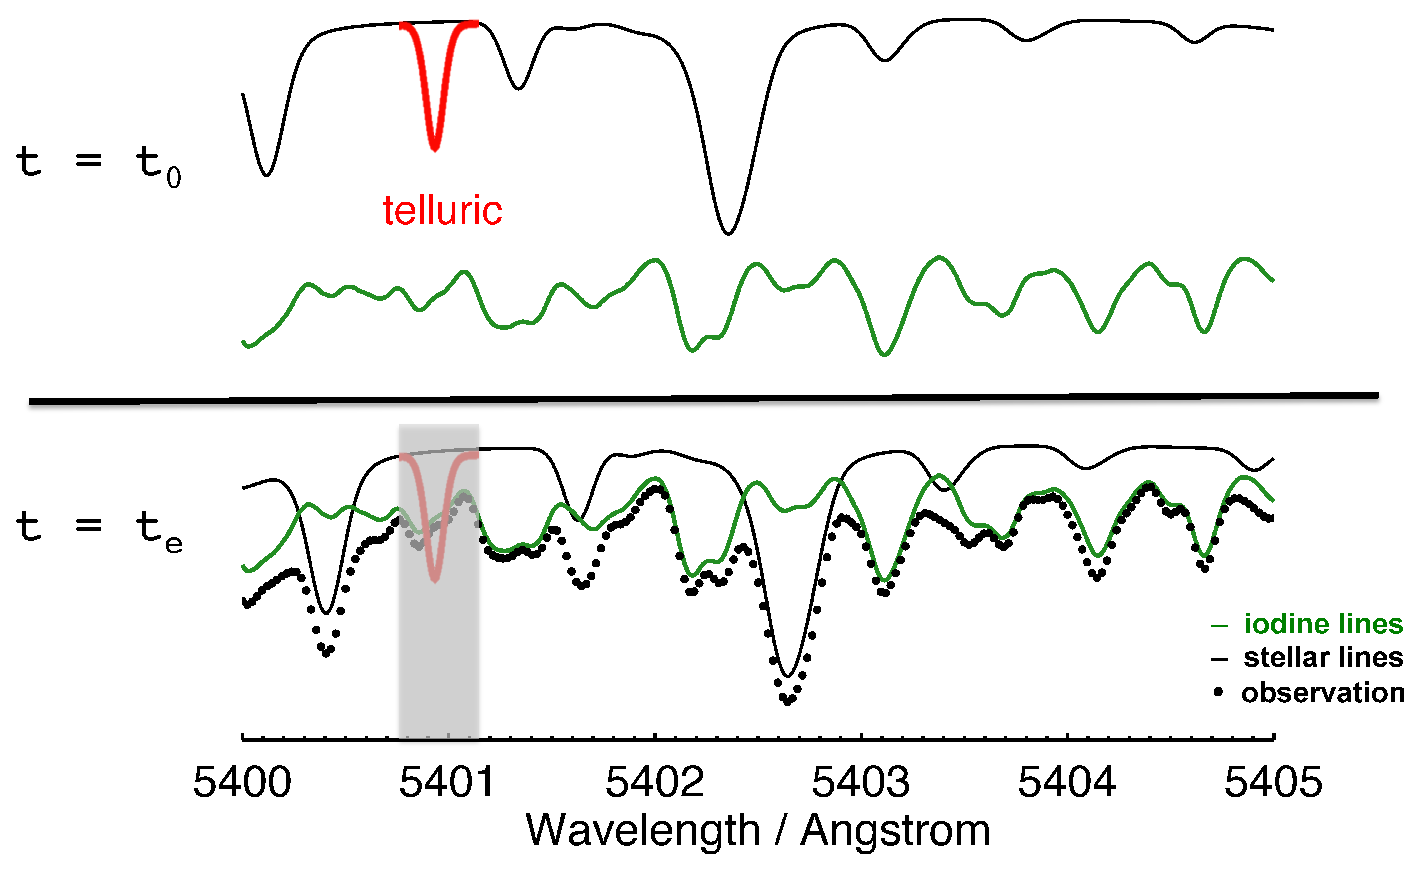
\includegraphics[scale=0.5]{telluric/dsst-mask1.eps}}\\
\subfloat{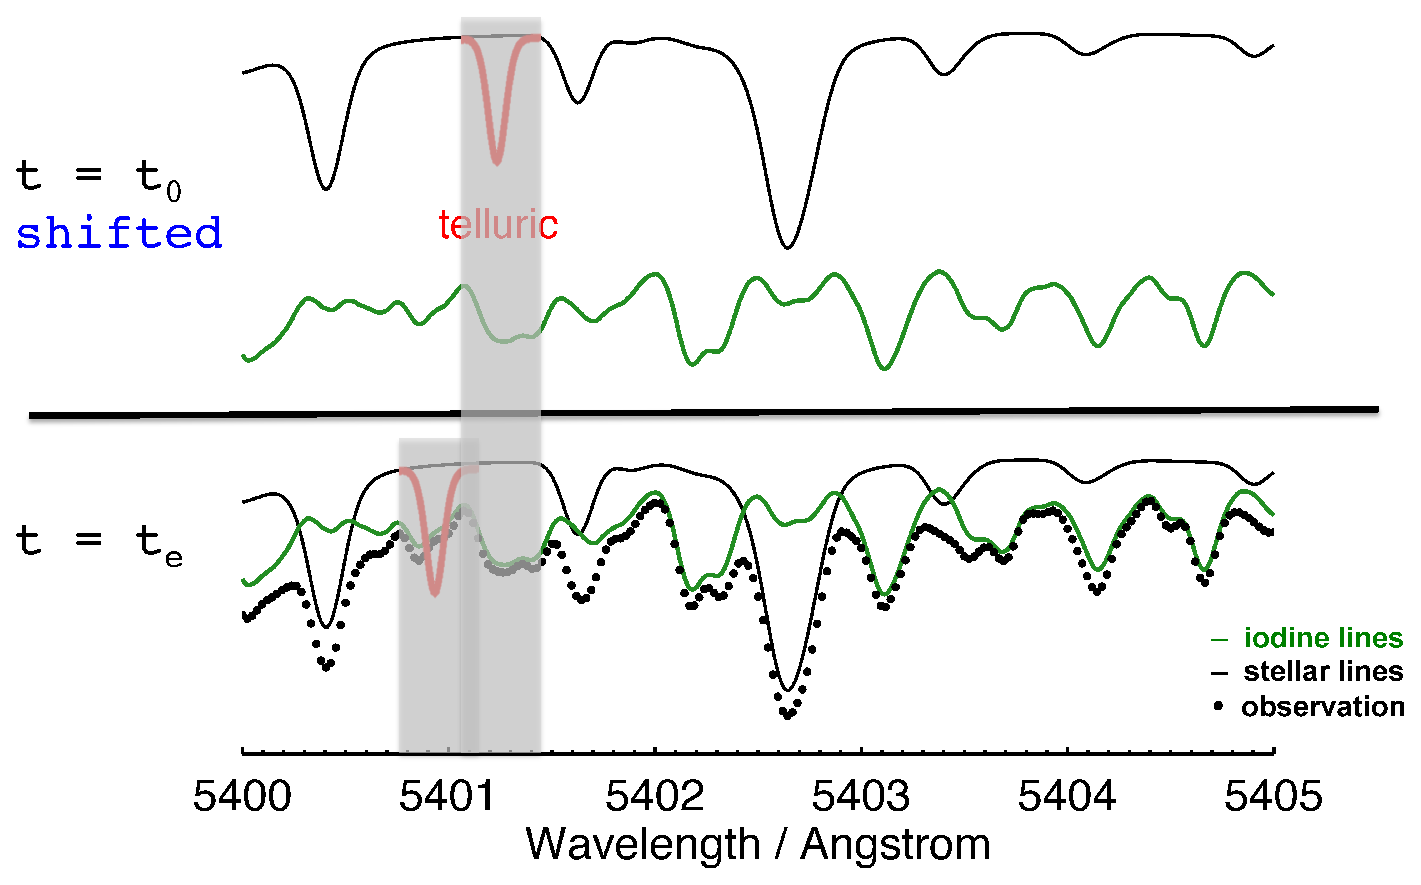
\includegraphics[scale=0.5]{telluric/dsst-mask2.eps}}
\caption{Illustration for how we mask telluric contaminated
pixels. The top panel shows how we mask the telluric lines (red solid
lines) in the epoch observation taken at $t=t_e$. The bottom panel
shows why we also need to mask pixels associated with telluric lines
in the deconvolved stellar reference spectrum taken at epoch $t=t_0$
and being shifted in order to model the observation.
\label{telluric:fig:dsstmask}}
\end{figure}
%----------------------------------------------------------------


% simulations and results 
To investigate the effectiveness of masking, we performed RV
extraction on simulated spectra with or without telluric lines
injected and with or without masking (all with Poisson noise and
complex IP to mimic real observations as much as possible). For
stellar reference spectrum, we used the synthetic spectrum with
telluric lines. The results are already listed in
Table~\ref{telluric:tab:simulation}, but is listed again in
Table~\ref{telluric:tab:rmsmasking} for clear comparisons. In terms of
improving RV precision or reducing RV RMS, masking is very
ineffective. The additional errors it introduces diminish its
merits. On the other hand, masking does improve the accuracy to some
degree: for example, masking does remove the downward RV trend seen in
HD 10700 data on the bottom right plot of
Figure~\ref{telluric:fig:sim} in the BC range $[-3\times10^4,\
-2\times10^4]$ m/s. However, masking is an ineffective way to mitigate
the effects of telluric contamination overall, especially since the RV
errors and RV-BC trends are dominated by photon noise and algorithmic
errors (and other types of errors too in real observations).

% why simple masking would not work for high precision/accuracy
So why masking does not work? First of all, it complicates the
$\chi^2$ surface and ``breaks'' the L-M fitter. Due to the ``dynamic''
nature of the mask mentioned above, the degrees of freedom for fitting
could change, because some telluric lines may shift in and out of this
spectral chunk as the wavelength solution changes. This would make the
fitter harder to converge or may create more loci for the fitter to
get stuck in, causing additional errors. Furthermore, masking is
throwing away iodine and stellar content embedded in these pixels
too. Finally, to ``mask'' the telluric lines out, one needs to pick a
flux threshold for the masks. This threshold must maintain a balance
between masking too much (throwing away too much iodine and stellar
information) and too little (leaving shallow telluric lines and line
wings untreated). In our study, we have chosen a flux threshold of
0.3\%, which means any pixel with telluric absorption deeper than
0.3\% will be masked (reference telluric spectrum is generated by
TERRASPEC at an altitude of 70$^{\degree}$, meaning deep oxygen lines,
and with pwv $=$ 0.8~mm, a little more than
typical \keck\ humidity). This masks 11\% of the spectral domain,
which is quite substantial and is very damaging to the RV precision,
but is almost the minimal amount of masking required to achieve some
RV accuracy improvement.

% how about masking in real observations?  
We also applied telluric masking in RV reduction for real
observations, and saw no improvement over RV precision or
accuracy. This is because other effects dominate rather than
tellurics, as mentioned above, such as photon and algorithmic errors
and especially deconvolution errors in stellar reference spectrum,
which are discussed in Section~\ref{keck:sec:dsst} and
\ref{keck:sec:algorithm}.

% summarize
To summarize, masking sounds like a simple solution to the problem of
micro-telluric contamination, but it is actually complicated to
implement (for iodine-calibrated RV reduction) and it is ineffective
in terms of improving RV precision. We do not recommend masking as a
remedy for treating micro-telluric lines in iodine-calibrated RV
work. We believe the most effective way is to forward model telluric
lines, and combine that with some ``masking'' for deep or troublesome
telluric lines, which we discuss in the next subsection.

\subsubsection{How precisely does one need to model the tellurics?}\label{keck:telluric:neid}


%----------------------------------------------------------------
% NEID Plot showing how much you need to model tellurics
\begin{figure}
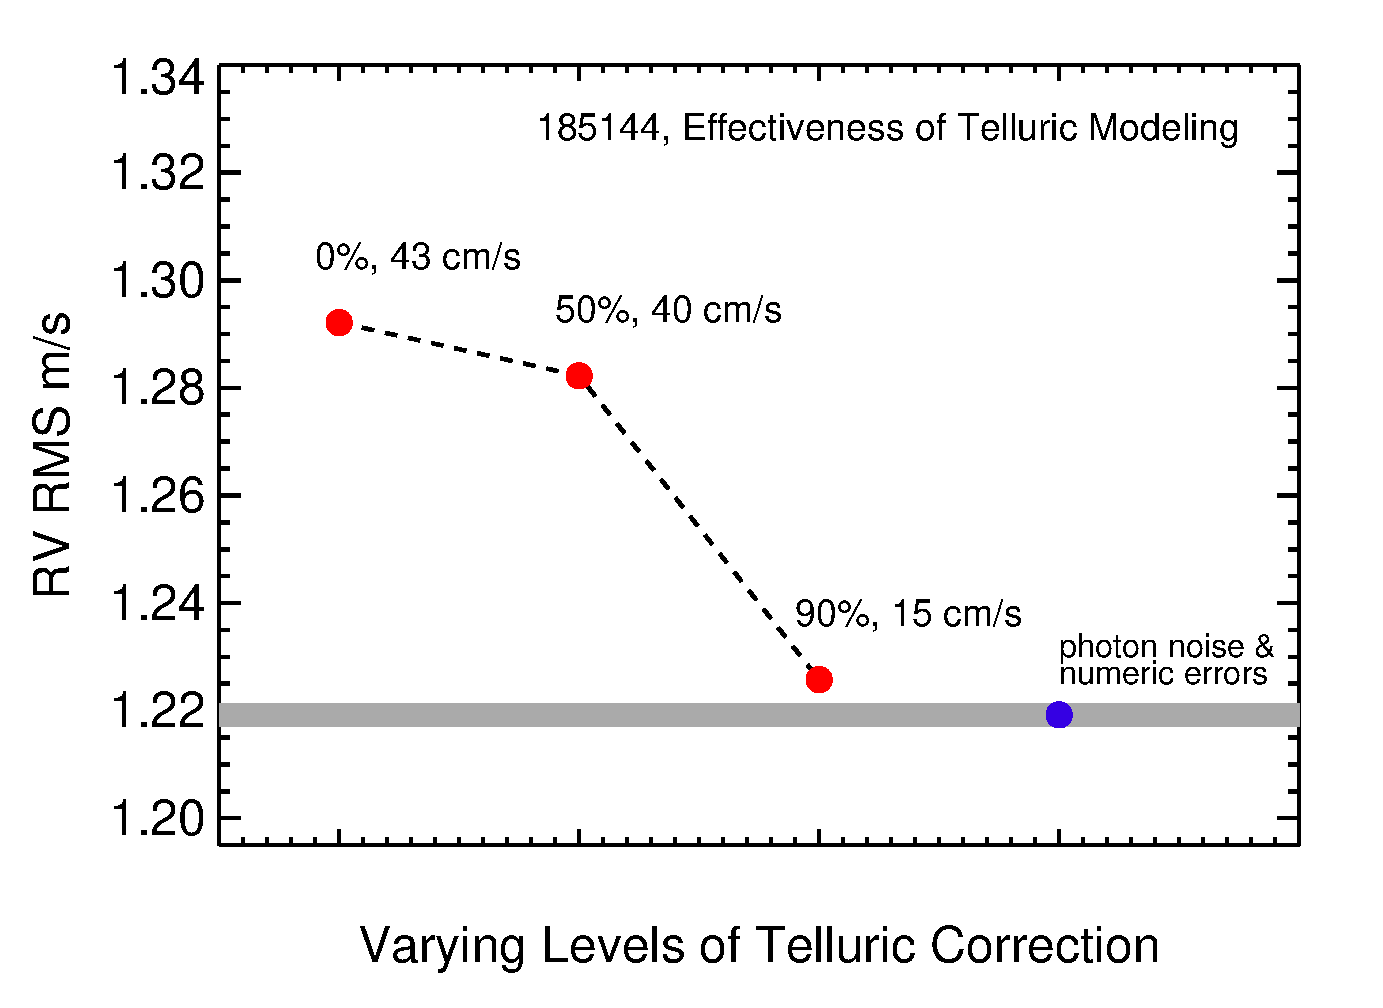
\includegraphics[scale=0.5]{telluric/neid.eps} 
\caption{Improvements in RV RMS for different ``level" of telluric
  modeling/removal. For example, the mid point labeled with ``50\%, 33 cm/s"
  means that if you model your telluric absorption lines to 50\% of
  their original depths, the effects of the residual telluric
  absorption will add 33 cm/s in quadrature to your final RV RMS. The
  blue point marks the RV RMS for simulations with Poisson noise and
  complex IP on HD 185144, which represents the photon-limited RV
  precision (subject to additional numeric or algorithmic errors; see
  Chapter~\ref{chap:conclusion} for more on the limitation of the
  Doppler code).
\label{telluric:fig:neid}}
\end{figure}
%----------------------------------------------------------------


% modeling is the way to go
The other way is to incorporate telluric lines as part of the iodine
RV forward modeling process, where water column density can either be
from a priori knowledge or an additional free parameter. In principle,
the oxygen column density can also be a free parameter, not because
the amount of oxygen varies on a noticeable level, but just to allow
some compensation for errors in atmospheric temperature and pressure
profile and so on. We do not fit for oxygen in our simulation or
treatment for real observations in this work for simplicity, and also
because the chunks contaminated with oxygen lines are in the reddest
part near 6300\AA, where the amount of iodine and stellar contents are
minimal anyway, and these chunks tend to be thrown away or heavily
de-weighted in the final RV weighting process.

% the goal of modeling
Modeling telluric absorption lines to high precision (below 1--2\% RMS
residual) can be a challenging task. There are several reasons for
this: lab measurements of a large number of water lines are
inaccurate, in terms of line depths, line positions, and line shapes;
and these line properties can also be uncertain due to change or a
lack of knowledge of the atmospheric conditions, such as wind, high
line-of-sight variations (e.g., water vapor), and mixing
uncertainties. For a summary of the state of the problem and paths
forward recommended by the RV community, see Section~4.6 in
\cite{eprv2015}. However, the goal here is not to model or ``remove''
the telluric lines perfectly, but to mitigate their impact on RV
precision and accuracy as much as possible. A central question is: how
well do we need to model telluric lines to reach a certain RV
precision \citep{eprv2015}?

% how well should we model?
To answer this question under the context of iodine-calibrated RV, we
performed RV extractions on the simulated HD 185144 data with telluric
absorption (all with pwv $=$ 1.0~mm, as described in
Section~\ref{keck:telluric:method}), incorporating forward modeling of
telluric lines with different levels of accuracy and using a stellar
reference spectrum free of tellurics. The results are illustrated in
Figure~\ref{telluric:fig:neid}. All three simulations were run with
simulated spectra of HD 185144 with pwv 1.0~mm, but the one labeled
``0\%'' has no telluric modeling in the RV extraction, while the one
labeled with ``50\%'' has synthetic telluric lines with pwv 0.5~mm in
the forward modeling process, and ``100\%'' meaning using telluric
model with pwv 1.0~mm, the same as the injected telluric lines. In
addition, we also used telluric model with pwv 1.1~mm in the forward
modeling, which basically produced the same RV RMS as the ``100\%''
simulation with no visible RV-BC trends or correlations. Extrapolating
between the results, a $\geq$90\% modeling accuracy for the water
lines would control the RV RMS contribution from tellurics to below
10~cm/s, which is near or beyond target precision for the next
generation RV spectrographs. This modeling is very easy to achieve in
reality.

% well actually vanking did a lot of heavy lifting
One important point to notice is that the reason why the damage of
10\% telluric modeling residual is controlled down to $\leq$10~cm/s is
the additional ``masking'' and weighting process in the Doppler code,
i.e., ``vanking'' (Chapter~\ref{chap:doppler}). In another word, a
combination of modeling (even only to 90\% precision) and statistical
weighting can effectively control the RV RMS introduced by tellurics
to $\leq$10~cm/s. Weighting plays a role in telluric contamination
remedy because it is essentially performing some ``masking'' on the
chunks that are badly contaminated by tellurics and/or have large
modeling residuals, such as the ones near 6300\AA\ with deep oxygen
lines and little stellar or iodine content.  Chunks with deep and
numerous oxygen lines are normally thrown out completely, and other
contaminated chunks which suffer from low precision will receive lower
weights and thus cast a lower impact on the final precision and
accuracy. In reality, we are using a combination of modeling and
masking or weighting to tackle problem of telluric contamination,
which we believe is the optimal solution for iodine-calibrated RVs.

\subsubsection{How about real observations?}\label{keck:telluric:real}

%----------------------------------------------------------------
% Effect of clean DSST and preliminary modeling with real data
% plot made by ~/Exo.../Keck.../plots_general/basic_rv.pro, choice='3panel'
\begin{figure}
\subfloat[HD 185144, rj82 template]{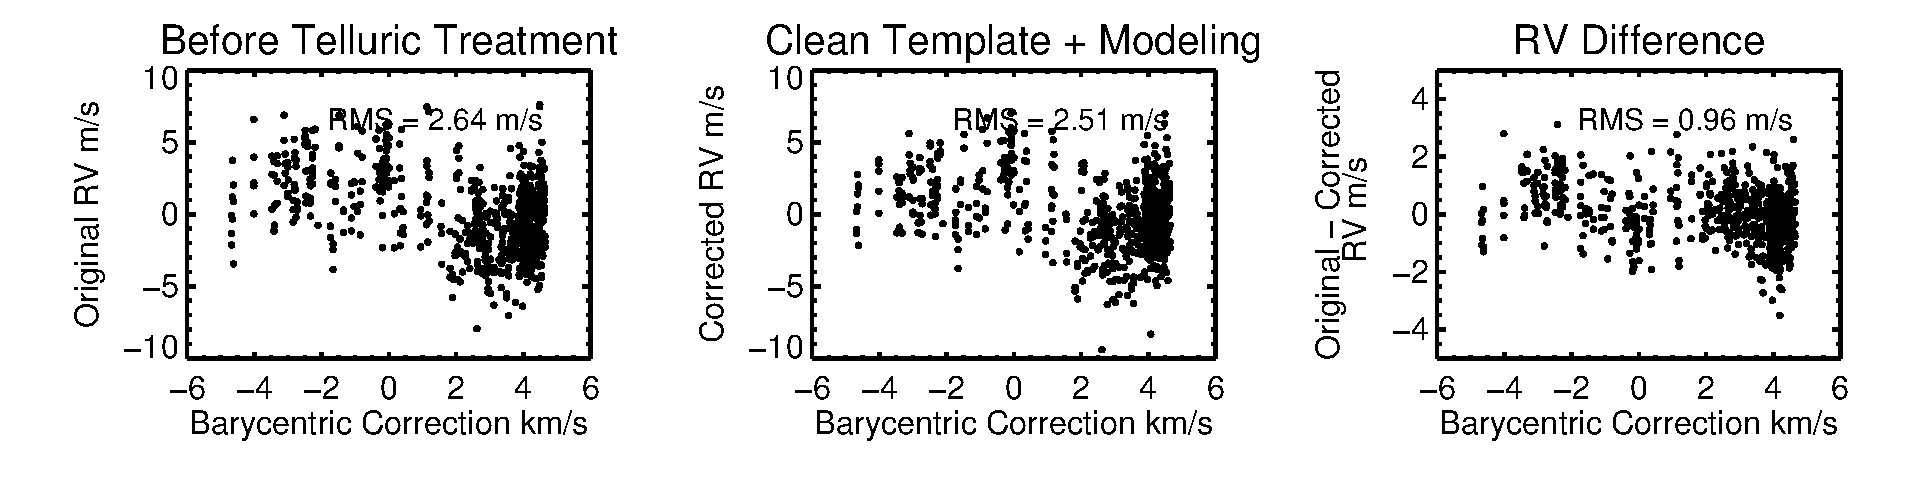
\includegraphics[scale=0.42]{telluric/185144_BC_RV_rj82_3panel.eps}}\
\subfloat[HD 185144, rj172 template]{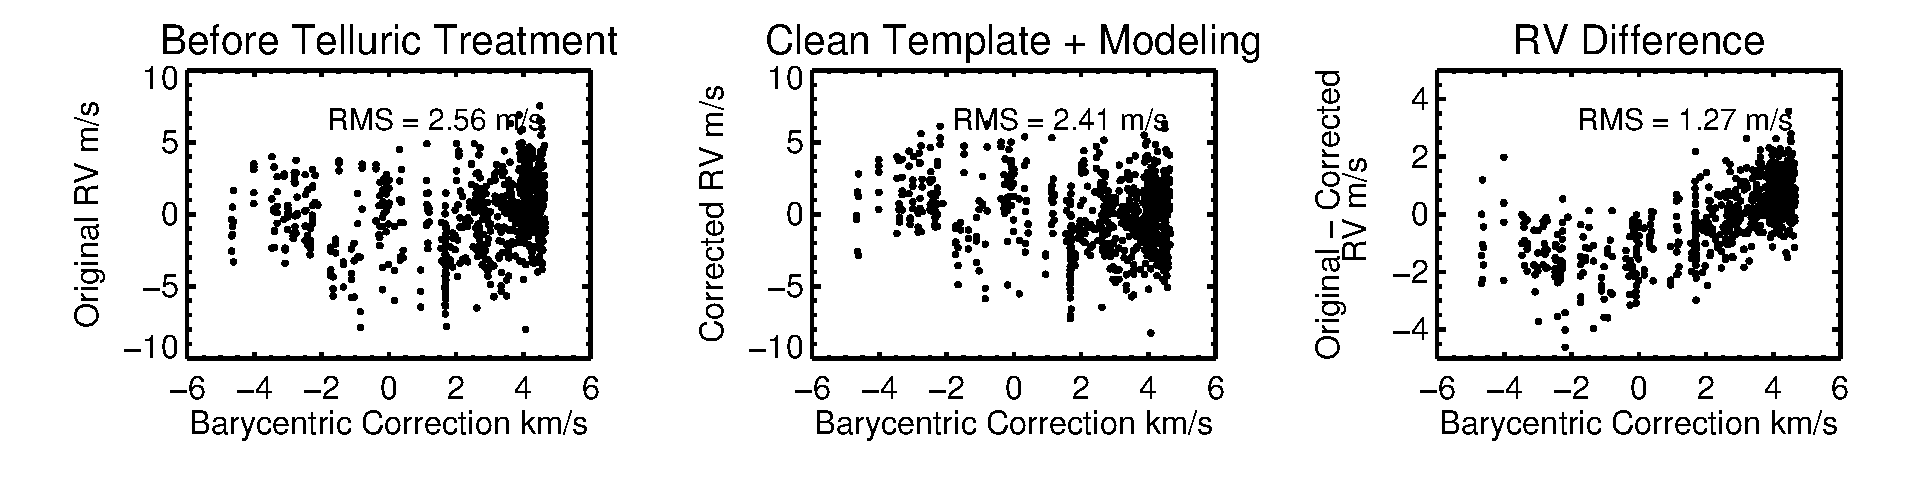
\includegraphics[scale=0.42]{telluric/185144_BC_RV_rj172_3panel.eps}}\
\subfloat[HD 10700, rj82 template]{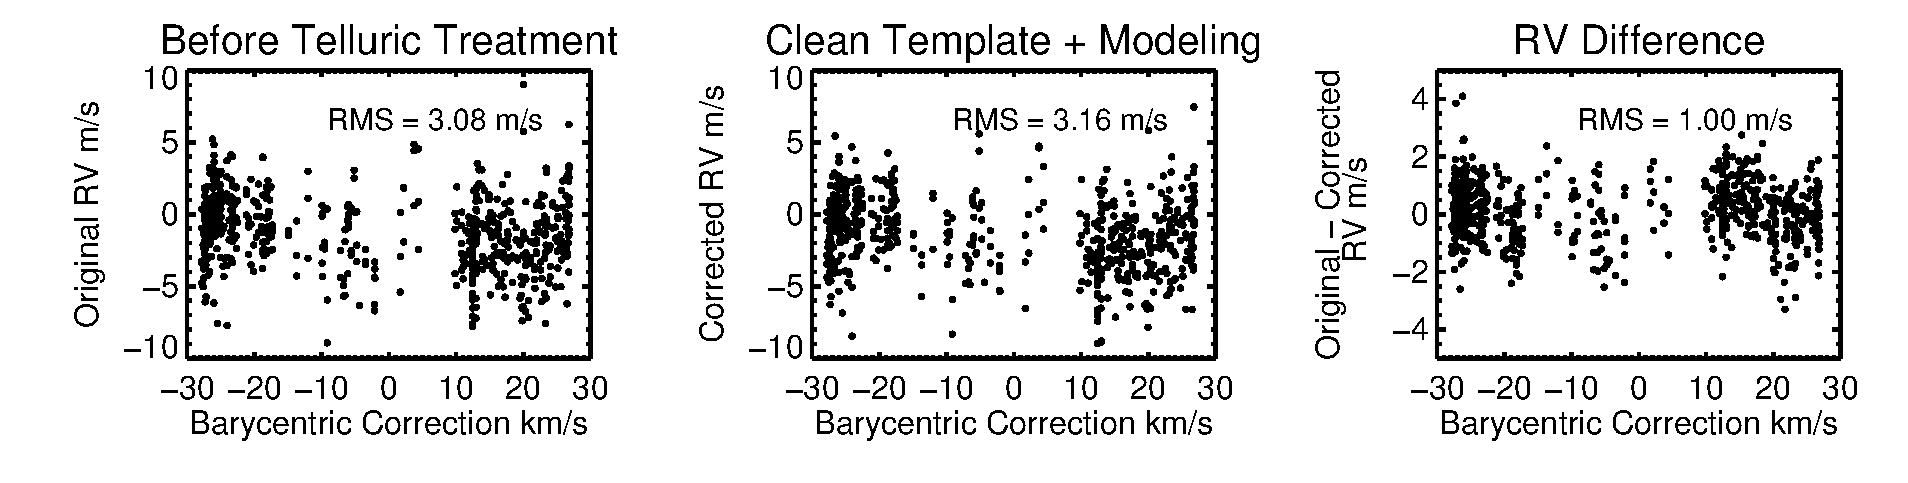
\includegraphics[scale=0.42]{telluric/10700_BC_RV_rj82_3panel.eps}}\
\caption{Effects of using clean DSST and preliminary telluric modeling
  on RV precision and accuracy, for HD 185144 (top two rows) and HD
  10700 (bottom row). There are two sets of data for HD 185144 because
  we ran the Doppler code with two DSSTs derived from spectra taken at
  two different epochs (i.e., at different BCs). The left and middle
  panels are showing RVs vs.\ BCs for RV extractions with and without
  telluric treatment, respectively. The right panels show the RV
  difference between the two panels.
\label{telluric:fig:real}}
\end{figure}
%----------------------------------------------------------------


% what should we do about real observations?
The situation is much more complicated for real observations, because
other noise sources enter the picture, some uncontrollable and/or
unknown. It turns out that telluric contamination is {\em not} the
dominant sources of RV systematic errors in \keck\ data. We later
found out that the major culprit behind the RV-BC correlation patterns
is probably errors in the DSSTs, which is discussed in
Section~\ref{keck:sec:dsst}. This fact makes it somewhat difficult to
assess the effectiveness of telluric treatment on real data, but the
simulations have demonstrated that the the best and effective strategy
is to have a clean DSST and to forward model the telluric lines (and
also to mask out deep lines and de-weight chunks with hard-to-clean
tellurics, which are already taken care of by vanking).

\begin{comment}
We have tested both masking and preliminary
modeling: In the case of HD 185144, RV RMS went down (from
2.57 m/s) after we applied masking (to 2.44 m/s) or modeling (to 2.50
m/s), with visible changes in the RV-BC trends. In the case of HD
10700, the RV RMS actually went up (from 3.05 m/s) after masking (to
3.26 m/s) or modeling (3.17 m/s), also with visible changes in the
RV-BC trend.
\end{comment}

% our best efforts...
Figure~\ref{telluric:fig:real} represents our best efforts so far and
their effects. Our treatment plan includes using ``cleaned'' DSSTs (we
describe how we cleaned the DSSTs later in this subsection) and
preliminary modeling of telluric lines in the Doppler code, where we
used pwv $=$ 1.0 mm for all observations instead of fitting pwv for
each one. In the case of HD 185144, the RV RMS values decreased after
we treated the tellurics, but it is not the case for HD 10700 -- we
suspect that the difference comes from the choice of the pwv value of
1~mm, which is more typical for HD 185144 observations but perhaps not
so for HD 10700 (these two stars are at very different
Declinations). We plan to model the water absorption in each
observation using best-fit or best-estimated pwv in the near future.

% DSST and how we cleaned it
How about telluric lines in the DSST? For simulations, we have the
privilege of using the synthetic spectrum which is naturally
telluric-free. For real observations, telluric contamination enters
every observed spectrum associated with the making of DSST (for a
detailed description of how the DSST is made, see
Section~\ref{doppler:sec:reference}). To remove errors in the DSST
caused by the telluric contamination, we formulated a recipe to
``clean up'' the DSST:

\begin{enumerate}
\item When fitting the bracketing B star $+$ iodine observations, we
  incorporate synthetic telluric lines generated by TERRASPEC as one of
  the input reference spectra (just like the iodine atlas). The water
  column density, or pwv, is determined by fitting two rich water bands
  among the spectrum taken by the red chip data of \keck\
  (7000-8000\AA). Although we use Mauna Kea's typical atmospheric
  condition and adjust oxygen column density according to observation
  altitude, we still fit for oxygen column density to allow some room
  for errors in the model (the adjustment needed is typically $<$0.5\%).
\item Using the IPs and wavelength solution derived in step (1), we
  run the deconvolution algorithm and generate a DSST, which would
  have telluric lines in it because telluric lines exist in the
  stellar (iodine-free) spectra.
\item We divide out the telluric lines in the DSST in two steps: 
  \begin{enumerate}
  \item Fitting two parameters to make sure the telluric lines match
    the ones in DSST: broadening parameter (width of a Gaussian
    kernel) and wavelength shift. The broadening parameter is
    necessary because the synthetic telluric lines are at an extremely
    high resolution, while the telluric lines in the DSST are
    deconvolved but are typically lower. The wavelength shift is
    needed because the wavelengths of the telluric lines, provided by
    the wavelength solution of the DSST, could differ from rest-frame
    telluric line wavelengths because of errors in DSST or changing
    atmospheric conditions such as wind. 
  \item Fitting these two parameters is not a straight forward
    least-$\chi^2$ problem, because stellar lines also present in the
    spectrum and we do not have an input model for them. Thus, instead
    of minimizing residuals between model (broadened and shifted
    telluric lines) and data (deconvolved telluric lines plus stellar
    lines), we minimize the flux above the continuum level to find
    best-fit parameters and the best-fit telluric model.
  \item We divide out the best-fit telluric model from the DSST to
    obtain a cleaned DSST.
  \end{enumerate}
\end{enumerate}

Naturally, this process does not clean up the DSST perfectly,
especially for deep and moderately deep lines, where the line profiles
are hard to match. We hope to improve this cleaning process, as well
as the entire process for making DSSTs, which we discuss in
Section~\ref{keck:sec:conclusion}. 


%%%%%%%%%%%%%%%%%%%%%%%%%%%%%%%%%%%%%%%%%%%%%%%%%%%%%%%%%%%%%%%%%%%%%%%%%%%%
%%%%%%%%%%%%%%%%%%%%%%%%%%%%%%%%%%%%%%%%%%%%%%%%%%%%%%%%%%%%%%%%%%%%%%%%%%%%
\subsection{Summary of Recommendations on Treating Telluric
  Contamination}\label{keck:telluric:summary} 

As argued and tested in the previous subsections, to effectively
eliminate the adverse effects of telluric contamination in
iodine-calibrated precise RV data, we recommend the following
strategies:
\begin{itemize}
  \item Masking deep and saturated lines and wings liberally, or
    deserting such spectral regions completely.
  \item Creating DSST following the recipe described in
    Section~\ref{keck:telluric:real}, i.e.\ modeling ``out'' telluric
    lines in every step. 
  \item Incorporating forward modeling of telluric lines in the RV
    extraction process.
  \item Assigning low statistical weights to RVs reported by
    telluric-contaminated spectral regions which suffer from low RV
    precision and accuracy.
\end{itemize}

We outline potential improvements and future works at the end of this
chapter in Section~\ref{keck:sec:conclusion}.